\section{有界变差函数的判别}

\subsection{直接使用定义判断}

\subsection{利用单调区间进行划分}
直觉上看, 有界变差函数不能
\begin{enumerate}
    \item 振荡得太狠(振幅大);
    \item 振荡得太频繁.
\end{enumerate}
而三角函数是最天然的振荡函数, 只要将$\sin x$中的$x$换一换就能调整频率, 而在$\sin x$前乘上一些函数则能控制振幅. 接下来是一系列关于三角函数的例子.
\begin{example}
    设
    $$f(x)=\begin{cases}
        \sin (1/x), & 0 < x \leq 1 \\
        0,          & x = 0,
    \end{cases}$$
    $f$是有界变差函数吗? 
\end{example}
\begin{solution}
    有界变差函数不能振荡得太频繁, 而当$x$距离$0$越来越近时, $1/x$会增加得越来越快, 从而包含的三角函数的周期区间就越来越多, 也即振荡得越来越频繁, 而且振幅恒为$1$! 有了这个直觉之后, 我们的目标就证明$f$不是有界变差函数. \\
    % 此处插入函数图像
    \begin{center}
    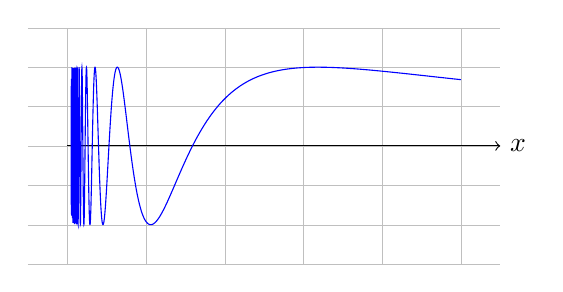
\begin{tikzpicture}[x=5cm]
    \draw[xstep=.2,ystep=.5,lightgray,ultra thin] (-0.1,-1.5) grid (1.1,1.5);
    \draw[->] (0,0) -- (1.1,0) node[right] {$x$};
    %\draw[->] (0,-1) -- (0,1.1) node[above] {$\sin (1/x)$};
    \draw[blue,domain=0.01:1,samples=5000] plot (\x, {sin((1/\x)r)});
    \end{tikzpicture}
    \end{center}
    虽然$\sin(1/x)$整体上振荡得图像都看不见了, 但是在局部上它与普通的三角函数$\sin x$没有本质区别: 在某个区间(即使非常短)内都要从$-1$单调增到$1$, 再单调减到$-1$. 
    记$y=1/x$, 则$\sin y$在$[2k\pi - \pi/2, 2k\pi + \pi/2]$上单调增, 在$[2k\pi + \pi/2, 2k\pi + 3\pi/2]$上单调减. 解不等式
    $$2k\pi - \frac{\pi}{2} \leq \frac{1}{x} \leq 2k\pi + \frac{\pi}{2}, \quad
      2k\pi + \frac{\pi}{2} \leq \frac{1}{x} \leq 2k\pi + \frac{3\pi}{2} $$
    得$\sin(1/x)$在$\displaystyle{\left[\frac{1}{2k\pi+\pi/2}, \frac{1}{2k\pi-\pi/2} \right] := [a_k, b_k]}$上单调增, 
    在$\displaystyle{\left[\frac{1}{2k\pi+3\pi/2}, \frac{1}{2k\pi+\pi/2} \right]} := [c_k, d_k]$上单调减.
    从右往左取分割点:
    $$1, b_1, a_1, d_1, c_1; b_2, a_2, d_2, c_2; \cdots $$
    但是有界变差函数定义中的分割只能有有限多个分割点, 所以我们取一列分割:
    \begin{align*}
        &\calP_1: 1, b_1, a_1, d_1, c_1; 0. \\
        &\calP_2: 1, b_1, a_1, d_1, c_1; b_2, a_2, d_2, c_2; 0. \\
        &\cdots \cdots \\
        &\calP_N: 1, b_1, a_1, d_1, c_1; \cdots; b_N, a_N, d_N, c_N; 0.
    \end{align*}
    在$[c_N, 0]$这一段显然有$|f(c_N)-f(0)| \leq 2\sup_{x\in [0,c_N]}|f(x)| \leq 2$. 在每个单调区间上, 有$|f(b_N)-f(a_N)|=|f(d_N)-f(c_N)|=2$, 所以$T_{\calP_N}(f) \geq 4N$. 也就是说, 对每个正整数$N$我们都能找到划分$\calP_N$使$f$在该划分下的全变差$\geq 4N$, 这就证明了$f$不是有界变差函数. 
\end{solution}                   
现在我们控制一下振幅:
\begin{example}
    设
    $$f(x)=\begin{cases}
        x^2 \sin (1/x), & 0 < x \leq 1 \\
        0,          & x = 0,
    \end{cases}$$
    $f$是有界变差函数吗?
\end{example}



%\begin{solution} % 此处解答错误, 后续更改
%    本例与上例唯一的不同之处在于单个单调区间上的估计:
%    $$|f(b_k)-f(a_k)| \leq \left|\frac{2}{(2k\pi - \pi/2)^2} \right|=O\Brace{\frac{1}{k^2}},$$ 类似地 $|f(d_k)-f(c_k)| \leq O\Brace{1/k^2}$. 最右端同样有$|f(1)-f(b_1)| \leq 2$,
%    所以$$T_{\calP_N}(f) \leq C\Sum{k=1}{N}\frac{1}{k^2}+4 \leq C\frac{\pi^2}{6}+4. $$
%    为何只需说明在\textbf{单调划分}下的变差有界就够了? 我们知道增加分割点会使变差增加(或不变), 现取定一个单调划分$\calP_N$, 往里添加一个分割点$t$:
%    \begin{enumerate}
%        \item 若$t \in (c_N, b_1)$, 则$t$必落在某个单调区间$[a_k,b_k]$(或$[c_k,d_k]$)内, 那么这一区间上的变差就要修正为
%        $$|f(b_k)-f(t)|+|f(t)-f(a_k)|=f(b_k)-f(t)+f(t)-f(a_k)=f(b_k)-f(a_k), $$
%        这与$\calP_N$对应的变差完全一样! 所以这个分割点加了和没加一样.
%        \item 若$t \in (b_1, 1)$, 理由同上(根据图像, $f$在$(b_1,1)$单调减). 
%        \item 如果$t \in (0, c_N)$, 我们要加入更多的单调区间把$t$盖进去. $t>0$意味着$t>\delta>0$, 而
%        $\displaystyle{c_k = \frac{1}{2k\pi + 3\pi/2} \to 0}$意味着存在$\Tilde{N}$使$c_{\Tilde{N}}<\delta<t$, 这样我们又回到了第一种情形, 且有
%        $$T_{\calP_N \cup \{t\}}(f) \leq T_{\calP_{\Tilde{N}}}(f) \leq C\frac{\pi^2}{6}+4.$$
%    \end{enumerate}
%\end{solution}



\begin{exercise} % Stein ex 3-11
    设$a,b>0$, 令
    $$f(x)=\begin{cases}
        x^a \sin (x^{-b}), & 0 < x \leq 1 \\
        0,          & x = 0,
    \end{cases}$$
    找出$f$是有界变差函数的充要条件.
    {[\textbf{提示}: 讨论$\displaystyle{\sum \frac{1}{k^{a/b}}}$的收敛性]}
\end{exercise}